
                \begin{figure}[H]
                    \centering
                    \begin{tikzpicture}
                        \pgfplotsset{%
                            width=1\textwidth,
                            height=0.4\textheight
                        }
                        \begin{axis}[
                            xlabel={Start battery level},
                            ylabel={Average dynamic energy (watt)},
                            ymin=0,ymax=20,
                        ]
                        
                            \addplot [mark=none, ultra thick, red]  coordinates {
                            (40, 13.078200713302017)(45, 13.333673736570914)(50, 13.205982190926816)(55, 13.142757098346694)(60, 13.136020817684509)(65, 13.405035569561575)(70, 13.04197328850529)(75, 12.94366076471958)(80, 11.865439322994966)
                            };
                            \addlegendentry{Surface4Pro - IntelPowerGadget}
                            
                            \addplot [mark=none, ultra thick, blue]  coordinates {
                            (40, 12.02162751922554)(45, 12.191671665720499)(50, 12.199436750403821)(55, 12.032581026957866)(60, 12.053564417718118)(65, 12.09948006642987)(70, 12.054071307650789)(75, 11.999796272264994)(80, 11.690016931934434)
                            };
                            \addlegendentry{Surface4Pro - HardwareMonitor}
                            
                            \addplot [mark=none, ultra thick, orange]  coordinates {
                            (45, 8.060371471492777)(50, 8.0502820332702)(55, 8.04648345457208)(60, 8.036646182097344)(65, 8.02575795361955)(70, 8.012424846710543)(75, 8.025221667057368)(80, 7.967618426220551)
                            };
                            \addlegendentry{Surface4Pro - RAPL}
                            
                            \addplot [mark=none, dashdotted, red]  coordinates {
                            (40, 3.240542599219406)(45, 3.502380761462297)(50, 3.483919670669171)(55, 3.580479783879264)(60, 3.4371081193211865)(65, 3.7378845804004857)(70, 4.1269371302643645)(75, 3.4284822260564574)(80, 3.8867754801290784)
                            };
                            \addlegendentry{SurfaceBook - IntelPowerGadget}
                            
                            \addplot [mark=none, dashdotted, blue]  coordinates {
                            (40, 3.246453721433944)(45, 3.8006481964613092)(50, 3.654884714881952)(55, 3.7283569264164593)(60, 3.7817250101807525)(65, 3.570805360389081)(70, 3.1888878694476537)(75, 3.9525756066315654)(80, 3.408293327314856)
                            };
                            \addlegendentry{SurfaceBook - HardwareMonitor}
                            
                            \addplot [mark=none, dashdotted, orange]  coordinates {
                            (40, 4.931648887847014)(45, 4.927856221494371)(50, 5.007900930165598)(55, 5.013531916608861)(60, 5.1503740837112355)(65, 5.152344821684819)(70, 5.296867745394305)(75, 5.50291940002461)(80, 5.612454815438993)
                            };
                            \addlegendentry{SurfaceBook - RAPL}
                            
                        \end{axis}
                    \end{tikzpicture} 
                \caption{A graph illustrating the energy consumption of Cores for test case BinaryTrees with regards to the battey level of the DUT (without outliers)} \label{fig:BinaryTrees_Cores_charge}
                \end{figure}
                